\documentclass{beamer}
\usepackage[french]{babel}
\usepackage{hyperref}
\definecolor{links}{HTML}{2A1B81}
\hypersetup{colorlinks,linkcolor=,urlcolor=links}
\usepackage{graphicx}
\usepackage{amsmath,amssymb}
\usepackage{tabularx}
\usepackage{booktabs}
\usepackage[compatibility=false]{caption}
\usepackage[toc,page]{appendix}
\usepackage{minted}
\usepackage{xspace}

\makeatletter
  \def\beamer@calltheme#1#2#3{%
    \def\beamer@themelist{#2}
    \@for\beamer@themename:=\beamer@themelist\do
    {\usepackage[{#1}]{\beamer@themelocation/#3\beamer@themename}}}

  \def\usefolder#1{
    \def\beamer@themelocation{#1}
  }
  \def\beamer@themelocation{}

\patchcmd{\minted@colorbg}{\noindent}{\medskip\noindent}{}{}
\apptocmd{\endminted@colorbg}{\par\medskip}{}{}
\makeatother

\newcolumntype{Y}{>{\centering\arraybackslash}X}

\usefolder{../theme}
\usetheme[numbering=fraction,block=fill,progressbar=frametitle]{metropolis} %Use metropolis theme

\definecolor{bg}{rgb}{0.95,0.95,0.95}
\setminted{bgcolor=bg,fontsize=\scriptsize,autogobble,mathescape,breaklines,tabsize=2}
\setmintedinline{breaklines,autogobble,fontsize=\scriptsize}
\setbeamersize{text margin left=8pt,text margin right=8pt}
\setbeamercovered{transparent}

\begin{document}

\title[C++]{Introduction à la programmation en C++}
\author[nicolas.audebert@onera.fr]{Nicolas Audebert}
\setmainfont{Fira Sans}


\AtBeginSection[]{
  \begin{frame}{Plan de la séance}
  \small \tableofcontents[currentsection]
  \end{frame}
}

\newcommand\cppi[1]{\mintinline{cpp}{#1}}
\newcommand\cpp[1]{%
  \begin{minted}{cpp}
  #1
  \end{minted}
}%

\author[nicolas.audebert@onera.fr]{Nicolas Audebert}
\date[24 nov. 2017]{Vendredi 24 novembre 2017}
\subtitle{Constructeurs - Destructeurs}
\maketitle

\begin{frame}{Avant toute chose}
  \begin{alertblock}{Rendus de TP et des exercices}
  Les rendus se font sur \href{https://educnet.enpc.fr}{\textbf{Educnet}}, même en cas de retard. \textbf{Pas par mail}.
  \begin{enumerate}
  	\item Le code rendu \textbf{doit compiler}.
    \item Le code rendu doit \textbf{être propre} (indentation, noms de variables clairs).
    \item Le code rendu doit \textbf{être commenté} (réponses aux questions, fonctionnement du code).
    \item Rassembler le code dans une seule archive (\texttt{.zip}, \texttt{.rar}, \texttt{.tar.gz}, etc.).
  \end{enumerate}
  Un exercice ou un TP rendu en retard ou ne respectant pas une des consignes ci-dessus sera pénalisé.
  \end{alertblock}
\end{frame}

\section{Rappels}

\begin{frame}[fragile=singleslide]{Les objets}
\begin{minipage}{0.48\linewidth}
    \begin{minted}{cpp}
    // Structure + fonctions
    struct Obj1{
        int x;
    };
    int f(Obj1 &x);
    int g(Obj1 &x, int y);

    ...
    Obj1 a;
    cout << f(a) << endl;
    int i = g(a,10);
    \end{minted}
\end{minipage}
\hfill
\begin{minipage}{0.48\linewidth}
    
        \begin{minted}{cpp}
// Objet
struct Obj1{
    int x;
    int f();
    int g(int y);
};

...
Obj1 a;
cout << a.f() << endl;
int i = a.g(10);
        \end{minted}
    
\end{minipage}

\vspace{0.3cm}
On met simplement les déclarations \textbf{dans} la structure.
\textbf{On ne met plus en argument} l'objet en question.
\end{frame}

\begin{frame}[fragile=singleslide]{Manipulation des objets}
Les objets se manipulent de façon similaire aux structures.

\begin{minipage}{0.50\linewidth}
    
        \begin{minted}{cpp}
struct Obj1{
  int x;
  void double_x();
  int renvoie_4x();
};

int main(){
  // En dehors de l'objet, on
  // utilise . pour accéder
  // aux champs et méthodes
  Obj1 a;
  a.x = 3;
  cout << a.renvoie_4x() << endl;
}
        \end{minted}
    
\end{minipage}
\hfill
\begin{minipage}{0.48\linewidth}
        \begin{minted}{cpp}
void Obj1::double_x(){
  // À l'intérieur du namespace
  // Obj1, on peut modifier ses champs
  x = 2*x;
}
int Obj1::renvoie_4x(){
  // À l'intérieur du namesapce
  // Obj1, on peut utiliser ses méthodes
  double_x();
  return x;
}
        \end{minted}
\end{minipage}
\end{frame}
\begin{frame}[fragile=singleslide]{Classes}
Les classes permettent de protéger l'accès à certains champs et méthodes afin de restreindre \textbf{l'interface} de l'objet.

    \begin{minted}{cpp}
// matrice.h
class Matrice{
  // privé par défaut
  int m,n;

public: // public à partir d'ici
  // Méthodes
  void cree(int m1,int n1);
  void detruit();
  double get(int i,int j);
  void set(int i,int j,double x);
  void affiche();

private: // privé à partir d'ici
    double* t;
};
    \end{minted}
\end{frame}

\section{Construction des objets}

\begin{frame}[fragile=singleslide]{Classes et structures}
    Séance précédente : structure + fonctions $\longrightarrow$ objets\\
    Par exemple :\\
    \begin{minipage}{0.38\linewidth}
        
            \begin{minted}{cpp}
struct Point{
    double x,y;
};
...
Point a;
a.x = 2; a.y = 3;
i = a.x; j = a.y;
            \end{minted}
        
    \end{minipage}
    \hfill
    \begin{minipage}{0.58\linewidth}
        
            \begin{minted}{cpp}
class Point{
    double x,y;
public:
    double get(double& x, double& y);
    void set(double valX, double valY);
}
...
Point a;
a.set(2,3);
a.get(i,j);
            \end{minted}
        
    \end{minipage}
\end{frame}

\begin{frame}[fragile=singleslide]{Initialisation d'une structure vs. initialisation d'un objet}
            \begin{minted}{cpp}
class Point{
    double x,y;
public:
    double get(double& x, double& y);
    void set(double valX, double valY);
}
...
Point a; // OK
a.set(2,3);
a.get(i,j);
...
Point b = {2,3};
// ERREUR
// x et y sont privés :
// ils sont inaccessibles en
// dehors de la classe
            \end{minted}
\end{frame}

\begin{frame}[fragile]{Notion de constructeur}
    \only<1>{L'initialisation d'un objet fait appel au \textbf{constructeur} de sa classe.}

    \begin{block}{Définition}
      Un \textbf{constructeur} est une méthode\,:
      \begin{itemize}
          \item qui \textbf{n'a pas} de type de retour,
          \item qui porte \textbf{le même nom} que la classe,
          \item qui décrit comment initialiser les instances de la classe.
      \end{itemize}
    \end{block}
    \begin{overprint}
    \onslide<1>
    \begin{alertblock}{Manipulation}
      Un constructeur :
      \begin{itemize}
          \item est \textbf{systématiquement} appelé à la création d'un objet,
          \item ne peut pas être appelé \textbf{après} la création de l'objet.
      \end{itemize}
    \end{alertblock}

    \onslide<2>
    \begin{minipage}{\linewidth}
    \begin{minipage}{0.59\linewidth}
            \begin{minted}{cpp}
class Point{
    double x,y;
public:
    Point(double valX, double valY);
    ...
}

// Définition du constructeur
Point::Point(double valX, double valY){
    x = valX; y = valY;
}
            \end{minted}
    \end{minipage}
    \hfill
    \begin{minipage}{0.39\linewidth}
            \begin{minted}{cpp}
...
Point b = {2,3}; // ERREUR
Point c(2,3); // OK
// Cette syntaxe appelle
// le constructeur
            \end{minted}
        
    \end{minipage}
    \end{minipage}
    \end{overprint}
\end{frame}

\begin{frame}[fragile=singleslide]{Le constructeur vide}
    À la création de l'objet il y a \textbf{toujours} un appel à un constructeur.

    Lorsqu'aucun constructeur n'est défini par l'utilisateur, le compilateur en créé un par défaut.
    C'est un \textbf{constructeur vide} qui ne prend aucun argument et ne fait que créer les champs de l'objet.
        \begin{minted}{cpp}
class Point{
    double x,y;
public:
    double get(double& x, double& y);
    void set(double valX, double valY);
};
...
Point a;// Appel au constructeur par défaut
        \end{minted}
    
\end{frame}

\begin{frame}[fragile=singleslide]{Redéfinir le constructeur vide}
    Il est possible de redéfinir le constructeur vide (dans ce cas, le constructeur par défaut est oublié).\\
    \begin{minipage}{0.44\linewidth}
            \begin{minted}{cpp}
class Point{
private:
    double x,y;
public:
    // Constructeur vide
    Point();

    double get(double& x,
               double& y);
    void set(double valX,
             double valY);
};
            \end{minted} 
    \end{minipage}
    \hfill
    \begin{minipage}{0.52\linewidth}
            \begin{minted}{cpp}
Point::Point(){
  cout << "Constructeur vide" << endl;
  x = 0; y = 0;
}

...
Point a; // "constructeur vide"
a.get(i,j);
cout << i << ", " << j << endl;
// affiche "0, 0"
            \end{minted}
    \end{minipage}
\end{frame}

\begin{frame}[fragile=singleslide]{Surchage des constructeurs}
    Il est possible de définir plusieurs constructeurs (comme pour les méthodes) manipulant différentes combinaisons d'arguments.

    \begin{minipage}{0.42\linewidth}
            \begin{minted}{cpp}
class Point{

    double x,y;
public:

    Point(double val);
    Point(double valX,
          double valY)
    ...
};
            \end{minted}
    \end{minipage}
    \hfill
    \begin{minipage}{0.56\linewidth}
            \begin{minted}{cpp}
Point::Point(double val){
    x = y = val;
}
Point::Point(double valX, double valY){
    x = valX; y = valY;
}

...
Point a(2); // 2 2
Point b(2,3); // 2 3

Point c; // ERREUR (pas de
         // constructeur vide)
            \end{minted}
    \end{minipage}
\end{frame}

\begin{frame}[fragile=singleslide]{Remplacement du constructeur vide}
    \begin{alertblock}{Attention !}
    Dès lors qu'un constructeur est défini, quel qu'il soit, \textbf{le constructeur par défaut n'existe plus}.
    \end{alertblock}

    Dans ce cas, il faut définir son propre constructeur vide pour pouvoir écrire \mintinline{cpp}{Point c;}.
    
        \begin{minted}{cpp}
class Point{
    double x,y;
public:
    Point();
    Point(double val);
    Point(double valX, double valY)
};
Point::Point(){} // Constructeur vide (ne fait rien)
        \end{minted}
    
\end{frame}

\begin{frame}[fragile=singleslide]{Constructeurs et tableaux d'objets}
    \begin{block}{Cas général}
        \textbf{Créer un tableau d'objets requiert l'existence du constructeur vide} pour cette classe d'objets.
    \end{block}
    
        \begin{minted}{cpp}
Point t[10]; // appelle 10 fois Point()
Point* t2 = new Point[1000]; // appelle 1000 fois Point()
//pour remplir :
for(int i=0; i<1000; i++)
    t2.set(0,0);
        \end{minted}
    
    \begin{exampleblock}{Cas particulier}
        Dans le cas d'une initialisation directe utilisant la syntaxe entre accolades \texttt{\{\}}, il est possible de se passer du constructeur vide.
    \end{exampleblock}
    
        \begin{minted}{cpp}
Point t[3] = {Point(0), Point(1,2), Point(5, -5)};
        \end{minted}
\end{frame}

\section{Objets temporaires}
\begin{frame}[fragile=singleslide]{Objets temporaires}
Certains objets sont créés puis meurent très rapidement\,:
    \begin{minted}{cpp}
void f(Point p){
    ...
}
Point g(){
    Point temp(1,2);
    return temp;
}

...
Point p1(5,6);
f(p1);

Point p2 = g();

Point p3 = g();
f(p3);
    \end{minted}
\end{frame}

\begin{frame}[fragile=singleslide]{Objets temporaires}
    Dans ce cas, il est préférable d'utiliser des objets temporaires anonymes pour éviter les recopies inutiles\,:
        \begin{minted}{cpp}
void f(Point p){
    ...
}
Point g(){
    return Point(1,2);
}

...
f(Point(5,6));
Point p2 = g();
f(g());

Point p3;
p3 = g();
p3 = Point(1,2);
        \end{minted}
\end{frame}

\begin{frame}[fragile=singleslide]{Erreur communes}
    Il ne faut pas abuser des objets temporaires.

    \begin{alertblock}{Les objets temporaires ne sont pas des accesseurs !}
            \begin{minted}{cpp}
    Point p3;
    p3 = g();
    ...
    p3 = Point(1,2); // moins efficace que p3.set(1,2)
            \end{minted}
    Dans \mintinline{cpp}{p3.set(1,2)} il n'y a pas de création d'objet temporaire.
    \end{alertblock}
    \begin{alertblock}{Les objets temporaires ne sont pas des constructeurs !}
        
            \begin{minted}{cpp}
    Point p4 = Point(1,2); // objet temporaire inutile
    Point p5(1,2); // on appelle le constructeur directement
            \end{minted} 
    \end{alertblock}
\end{frame}

\begin{frame}[fragile=singleslide]{Exemple d'utilisation d'objet temporaire}
    \begin{minipage}{0.47\linewidth}
    
        \begin{minted}{cpp}
class Point{
    ...
    Point operator+(Point b);
};
Point Point::operator+(Point b){
    Point c(x+b.x, y+b.y);
    return c;
    // on retourne la copie de c
}
Point p1(1,2), p2(3,4);
Point p3 = p1 + f(p2);
        \end{minted}
    \end{minipage}
    \hfill
    \begin{minipage}{0.47\linewidth}
    
        \begin{minted}{cpp}
class Point{
    ...
    Point operator+(Point b);
};

Point Point::operator+(Point b){
    return Point(x+b.x, y+b.y);
    // on retourne l'objet
    // temporaire
}

Point p3 = Point(1,2) + f(Point(3,4));
        \end{minted}
    \end{minipage}
\end{frame}

\section{Passage par référence constante}

\begin{frame}{Rappel : le passage par référence}
    Une fonction peut recevoir ses arguments de deux manières\,:
    \begin{block}{Passage par valeur (ou copie)}
        La fonction reçoit une \textbf{copie} interne de la variable en argument.
    \end{block}
    \begin{block}{Passage par référence}
        L'e\textbf{space mémoire de la variable est partagé} et modifier l'argument dans la fonction modifie la valeur de la variable initiale.
    \end{block}
\end{frame}

\begin{frame}[fragile=singleslide]{Réduire le nombre de copies}
    Passer un argument par valeur nécessite de réaliser une copie. Copier un objet ou une variable ajoute un surcoût négligeable pour les variables natives, mais important pour les grands objets.

    \begin{minipage}{0.46\linewidth}
            \begin{minted}{cpp}
const int N = 1000;
class Vector{
    double t[N];
    ...
};
class Matrix{
    double t[N][N];
    ...
};
            \end{minted}
    \end{minipage}
    \hfill
    \begin{minipage}{0.48\linewidth}
            \begin{minted}{cpp}
void solve(Matrix A, Vector x,
           Vector& y)
{...}

...
Matrix M;
Vector a,b;
...
solve(M,a,b);
            \end{minted}
    \end{minipage}

\vspace{0.2cm}
La matrice \texttt{\textbf{M}} est copiée lors de l'appel à \texttt{\textbf{solve}}.

\end{frame}

\begin{frame}[fragile=singleslide]{Tout passer par référence ?}
Une solution serait de passer tous les arguments par référence pour éviter les copies.

    \begin{minipage}{0.44\linewidth}
            \begin{minted}{cpp}
const int N = 1000;
class Vector{
    double t[N];
    ...
};
class Matrix{
    double t[N][N];
    ...
};
            \end{minted}
    \end{minipage}
    \hfill
    \begin{minipage}{0.50\linewidth}
            \begin{minted}{cpp}
void solve(Matrix &A,Vector &x,Vector& y)
{...}

...
Matrix M;
Vector a,b;
...

solve(M,a,b);
            \end{minted}
    \end{minipage}

\begin{alertblock}{Risque}
    Rien ne garantit que \texttt{\textbf{solve}} ne modifie pas les arguments.
\end{alertblock}
\end{frame}

\begin{frame}[fragile=singleslide]{Référence constantes}
    \begin{block}{Solution}
        On souhaite passer les objets par référence en spécifiant que l'argument ne doit pas être modifié: \textbf{on ajoute le mot clé \texttt{const}}.
    \end{block}
    \begin{minipage}{0.44\linewidth}
            \begin{minted}{cpp}
const int N = 1000;
class Vector{
    double t[N];
    ...
};
class Matrix{
    double t[N][N];
    ...
};
            \end{minted}
    \end{minipage}
    \hfill
    \begin{minipage}{0.50\linewidth}
            \begin{minted}{cpp}
void solve(const Matrix &A,
    const Vector &x, Vector& y)
{...}

...
Matrix M;
Vector a,b;
...
solve(M,a,b);
            \end{minted}
    \end{minipage}
\end{frame}

\begin{frame}[fragile=singleslide]{Méthodes constantes}
    Lorsqu'on utilise une référence constante, on ne peut accéder qu'aux méthodes définies comme \textbf{constantes}, \textit{i.e.} qu'on a déclaré comme ne modifiant pas l'objet.

    \begin{minipage}{0.44\linewidth}
            \begin{minted}{cpp}
const int N = 1000;
class Vector{
    double t[N];
public
    double get(int i);
    void set(int i, double v);
    ...
};
class Matrix{
    double t[N][N];
    ...
};
            \end{minted}
    \end{minipage}
    \hfill
    \begin{minipage}{0.50\linewidth}       
            \begin{minted}{cpp}
void solve(const Matrix &A,
    const Vector &x, Vector& y)
{
    ...
    x.set(10, 8); // ERREUR: x est
                  // non modifiable
    x.get(5); // ERREUR

    y.set(1, 5.6); // OK
}
...
            \end{minted}
    \end{minipage}
\end{frame}


\begin{frame}[fragile=singleslide]{Méthodes constantes}
    Lorsqu'on utilise une référence constante on accès qu'au méthodes définies comme \textbf{constantes}: \textit{i.e.} qu'on a déclaré comme ne modifiant pas l'objet.

    \begin{minipage}{0.48\linewidth}
            \begin{minted}{cpp}
const int N = 1000;
class Vector{
    double t[N];
public
    double get(int i) const;
    void set(int i, double v);
    ...
};

double Vector::get(int i) const{
    return t[i];
}

            \end{minted}
        
    \end{minipage}
    \hfill
    \begin{minipage}{0.50\linewidth}
        
            \begin{minted}{cpp}
void solve(const Matrix &A,
    const Vector &x, Vector& y)
{
    ...
    x.set(10, 8); // ERREUR: x est
                  // non modifiable
    x.get(5); // OK, get est const

    y.set(1, 5.6); // OK
}

...
            \end{minted}
        
    \end{minipage}

\end{frame}

\section{Destructeurs}

\begin{frame}{Propriétés d'un destructeur}
    La création d'un objet appelle un constructeur.
    
    La supression d'un objet appelle un \textbf{destructeur}.

    \begin{block}{Définition et propriétés}
    Un destructeur est une méthode qui :
    \begin{itemize}
        \item n'a pas de type de retour,
        \item n'a pas d'argument,
        \item porte le nom de la classe précédé de \mintinline[fontsize=\large]{cpp}{~} (tilde).
    \end{itemize}
    \end{block}
\end{frame}

\begin{frame}[fragile=singleslide]{Implémentation des destructeurs}
    \begin{block}{Propriétés des destructeurs}
    Un destructeur est\,:
    \begin{itemize}
        \item unique pour chaque classe,
        \item fourni par défaut par remplaçable,
        \item \textbf{JAMAIS} appelé explicitement.
    \end{itemize}
    \end{block}

    \begin{minipage}{0.48\linewidth}
            \begin{minted}{cpp}
class Obj{
    ...
public:
    Obj(); // constructeur vide
    Obj(int i);

    ~Obj(); // destructeur
    ...
};
            \end{minted}
    \end{minipage}
    \hfill
    \begin{minipage}{0.50\linewidth}
            \begin{minted}{cpp}
Obj::~Obj(){

    cout << "Destruction";
    cout << endl;

}
            \end{minted}
    \end{minipage}
\end{frame}

\begin{frame}[fragile=singleslide]{Destructeurs et tableaux}

    Le destructeur est appelé autant de fois qu'il y a d'éléments dans le tableau.
    
        \begin{minted}{cpp}
{
    Obj tab[100]; // appel 100 fois au constructeur vide
    ...
} // sortie de bloc : destruction de tab -> 100 appels au destructeur
        \end{minted}
    
    En allocation dynamique, le destructeur est appelé lors du \mintinline{cpp}{delete}.
    
        \begin{minted}{cpp}
Obj* tab2 = new Obj[10000]; // 10000 appels au constructeur vide
...
delete[] tab2; // 10000 appels au destructeur de Obj
        \end{minted}
    
\end{frame}

\begin{frame}[fragile=singleslide]{Destructeurs et tableaux}
    
        \begin{minted}{cpp}
Obj* tab2 = new Obj[10000]; // 10000 appels au constructeur vide
...
delete[] tab2; // 10000 appels au destructeur de Obj
        \end{minted}
    
\begin{alertblock}{Attention erreur}
    Il est possible d'écrire \mintinline{cpp}{delete tab2}.
    Cela désalloue la mémoire mais n'appelle pas le destructeur sur les objets !
\end{alertblock}
\end{frame}

\section{Constructeur de copie}

\begin{frame}[fragile=singleslide]{Constructeur de copie}

    Le constructeur de copie permet de créer un objet à partir d'un autre.
            \begin{minted}{cpp}
class Obj{
    ...
    Obj(const Obj& o);
};
Obj::Obj(const Obj& o){...}
            \end{minted}
        
    Il s'utilise quand on écrit :
    
\begin{minipage}{0.45\linewidth}
            \begin{minted}{cpp}
Obj a;
Obj b(a);
            \end{minted}
\end{minipage}
\begin{minipage}{0.45\linewidth}
            \begin{minted}{cpp}
Obj a;
Obj b = a;
// c'est la même syntaxe que Obj b(a);
            \end{minted}
\end{minipage}

    Il est aussi implicitement utilisé lorsque l'on passe un objet par copie en argument d'une fonction.
\end{frame}

\begin{frame}{Constructeur de copie}
    \begin{block}{Définition}
    \begin{itemize}
        \item Un constructeur de copie est fourni par défaut
        \item Par défaut il recopie les champs de \texttt{a} dans \texttt{b}
        \item Une fois redéfini, il fait \textbf{uniquement} ce qu'il y a dans la méthode.
    \end{itemize}
    \end{block}
\end{frame}

\section{Opérateur d'affectation (=)}

\begin{frame}[fragile=singleslide]{L'opérateur d'affectation}
    Il est aussi possible de redéfinir l'opération d'affectation, le \texttt{=}.\\
    Par défaut, il recopie les champs d'un objet dans l'autre.
    
        \begin{minted}{cpp}
class Obj{
    ...
    void operator=(const Obj& o);
};
void Obj::operator=(const Obj& o){...}
        \end{minted}
\end{frame}

\begin{frame}[fragile=singleslide]{Opérateur =}
    
        \begin{minted}{cpp}
class Obj{
    ...
    void operator=(const Obj& o);
};
void Obj::operator=(const Obj& o){...}

Obj a,b;
b = a; // OK
Obj c;
c = b = a; // ERREUR
        \end{minted}
    
    Il faut lire :
    
        \begin{minted}{cpp}
Obj a,b,c;
c = b = a; // équivalent à
c = (b = a); // ou encore
c.operator=(b.operator=(a));
        \end{minted}
    
    \mintinline{cpp}{operator=} est de type \mintinline{cpp}{void} !
\end{frame}

\begin{frame}[fragile=singleslide]{Opérateur =}
    
\begin{minipage}{0.48\linewidth}
        \begin{minted}{cpp}
class Obj{
    ...
    Obj operator=(const Obj& o);
};
Obj Obj::operator=(const Obj& o){
    ...
    return o;
}
\end{minted}
\end{minipage}
\hfill
\begin{minipage}{0.46\linewidth}
\begin{minted}{cpp}
Obj a,b;
b = a; // OK
Obj c;
c = b = a; // OK
        \end{minted}
\end{minipage}

Pour éviter une recopie supplémentaire au niveau du \mintinline{cpp}{return} :
    \begin{minted}{cpp}
class Obj{
    ...
    const Obj& operator=(const Obj& o);
};
const Obj& Obj::operator=(const Obj& o){
    ...
    return o;
}
    \end{minted}

\end{frame}

\begin{frame}{Avertissement}
    \begin{alertblock}{Attention !}
        Il ne faut jouer aux apprentis sorciers. Ce n'est pas la peine de recoder le destructeur et le construteur par copie lorsque cela n'est pas nécessaire.
    \end{alertblock}
\end{frame}

\section{Objets avec allocation dynamique}

\begin{frame}[fragile=singleslide]{Une classe de vecteur}
    \begin{minipage}{0.44\linewidth}
            \begin{minted}{cpp}
class Vect{
    int n;
    double* t;
public:
    Vect(int taille);
    ~Vect();
};
            \end{minted}
    \end{minipage}
    \hfill
    \begin{minipage}{0.50\linewidth}
            \begin{minted}{cpp}
Vect::Vect(int taille){
    n = taille;
    t = new double[n];
}
Vect::~Vect(){
    delete[] t;
}
            \end{minted}
    \end{minipage}
    
        \begin{minted}{cpp}
void f(){
    Vect v(1000); // contructeur -> allocation
    ...
} // destructeur -> desallocation
        \end{minted}
    
Plus besoin de faire les \mintinline{cpp}{new} et les \mintinline{cpp}{delete[]} à la main.
\end{frame}

\begin{frame}[fragile=singleslide]{Une classe de vecteur}
    \textbf{Petit problème :} si on veut faire des tableaux de \texttt{Vect}, ou si on donne une taille négative ou nulle.

    \begin{minipage}{0.44\linewidth}
        
            \begin{minted}{cpp}
class Vect{

    int n;
    double* t;

public:

    Vect();

    Vect(int taille);

    ~Vect();

};
            \end{minted}
        
    \end{minipage}
    \hfill
    \begin{minipage}{0.50\linewidth}
        
            \begin{minted}{cpp}
Vect::Vect(){
    n = 0;
}
Vect::Vect(int taille){
    if(taille > 0){
        n = taille;
        t = new double[n];
    } else {
        n = 0;
    }
}
Vect::~Vect(){
    if(n > 0){
        delete[] t;
    }
}
            \end{minted}
        
    \end{minipage}
\end{frame}

\begin{frame}[fragile=singleslide]{Une classe de vecteur}
    \textbf{Un autre problème :} le code suivant ne fonctionne pas.

\begin{minipage}{0.44\linewidth}    
        \begin{minted}{cpp}
int main(){
    Vect v1(100), v2(100);
    v1 = v2; // fuite de mémoire
    return 0;
}

class Vect{
    int n;
    double* t;
public:
    Vect();
    Vect(int taille);
    ~Vect();
    const Vect& operator=(
            const Vect& v);
};
            \end{minted}
        
    \end{minipage}
    \hfill
    \begin{minipage}{0.50\linewidth}
            \begin{minted}{cpp}
const Vect& Vect::operator=
            (const Vect& v){
    if(n>0)
        delete[] t;
    n = v.n;
    if(n>0){
        t = new double[n];
        for(int i=0; i<n; i++)
            t[i] = v.t[i];
    }
    return v;
}
            \end{minted}
    \end{minipage}

    Ce code ne fonctionne pas si on fait \texttt{v=v}. (désallocation puis lecture dans une zone qui n'existe plus)
\end{frame}

\begin{frame}[fragile=singleslide]{Une classe de vecteur}

    \begin{minipage}{0.44\linewidth}
        
            \begin{minted}{cpp}
class Vect{
    int n;
    double* t;
    void alloue(int taille);
    void detruit();
    void copie(const Vect& v);
public:
    Vect();
    Vect(const Vect& v);
    ~Vect();
    const Vect& operator=(
        const Vect& v);
    Vect(int taille);
};
            \end{minted}
        
    \end{minipage}
    \hfill
    \begin{minipage}{0.50\linewidth}
        
            \begin{minted}{cpp}
void Vect::alloue(int taille){
    if(taille > 0){
        n = taille;
        t = new double[n];
    } else {
        n = 0;
    }
}
void Vect::detruit(){
    if(n > 0)
        delete[] t;
}
void Vect::copie(const Vect& v){
    alloue(v.n);
    for(int i=0; i<n; i++)
        t[i] = v.t[i];
}
            \end{minted}
        
    \end{minipage}
\end{frame}

\begin{frame}[fragile=singleslide]{Une classe de vecteur}

    \begin{minipage}{0.44\linewidth}
        
            \begin{minted}{cpp}
class Vect{
    int n;
    double* t;
    void alloue(int taille);
    void detruit();
    void copie(const Vect& v);
public:
    Vect();
    Vect(const Vect& v);
    ~Vect();
    const Vect& operator=(const
                Vect& v);
    Vect(int taille);
};
            \end{minted}
        
    \end{minipage}
    \hfill
    \begin{minipage}{0.50\linewidth}
        
            \begin{minted}{cpp}
Vect::Vect(){
    alloue(0);
}
Vect::Vect(const Vect& v){
    copie(v);
}
Vect::~Vect(){
    detruit();
}
const Vect& Vect::operator=(
        const Vect& v){
    if(this != &v){
        detruit();
        copie(v);
    }
    return v;
}
Vect::Vect(int taille){
    alloue(taille);
}
            \end{minted}
        
    \end{minipage}
\end{frame}

\begin{frame}{TP}
    \begin{minipage}{0.47\linewidth}
        \begin{block}{Serpent}
            Un serpent qui se déplace et s'allonge tout les \texttt{x} pas de temps.
        \end{block}
            \begin{block}{Tron}
                Un serpent deux joueurs qui s'allonge à tous les pas de temps.
            \end{block}

    \end{minipage}
    \hfill
    \begin{minipage}{0.47\linewidth}
        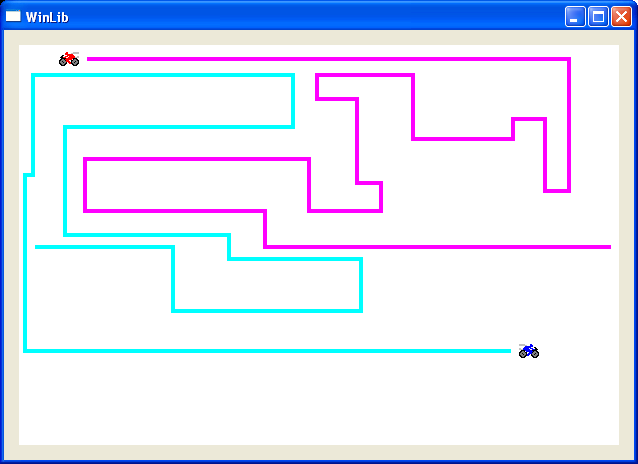
\includegraphics[width=\linewidth]{images/tp.png}
    \end{minipage}
\end{frame}

\end{document}
